\documentclass[twoside]{article}

\usepackage{ustj}
\usepackage{subcaption}

\addbibresource{mss.bib}

\newcommand{\authorname}{K. Afonin}
\newcommand{\authorpatp}{\patp{dozreg-toplud}}
\newcommand{\affiliation}{~}

%  Make first page footer:
\fancypagestyle{firststyle}{%
\fancyhf{}% Clear header/footer
\fancyhead{}
\fancyfoot[L]{{\footnotesize
              %% We toggle between these:
              % Manuscript submitted for review.\\
              {\it Urbit Systems Technical Journal} I:1 (2024):  133–150. \\
              ~ \\
              Address author correspondence to \authorpatp.
              }}
}
%  Arrange subsequent pages:
\fancyhf{}
\fancyhead[LE]{{\urbitfont Urbit Systems Technical Journal}}
\fancyhead[RO]{\texttt{urwasm} WebAssembly Interpreter Suite}
\fancyfoot[LE,RO]{\thepage}

%%MANUSCRIPT
\title{The \texttt{urwasm} WebAssembly Interpreter Suite on Urbit}
\author{\authorname~\authorpatp \\ \affiliation}
\date{}

\begin{document}

\maketitle
\thispagestyle{firststyle}

\begin{abstract}
\noindent
WebAssembly is a low-level language for a portable virtual machine. Wasm is designed to be a compilation target for a variety of programming languages and its design is hardware independent and relatively simple, making its support ubiquitous in modern browsers. Its simple design made it a perfect first candidate for a first emulator of an conventional computational system on a novel functional computer: Urbit. In this paper I discuss the current state of the \texttt{urwasm} project and some technical details, as well as describe the strategy to jet the interpreter of a state machine in a functional environment.
\end{abstract}

% We will adjust page numbering in final editing.
\pagenumbering{arabic}
\setcounter{page}{133}

\tableofcontents

\section{Introduction}

\begin{quote}
\ldots{} Martian code is so perfect that it cannot be contaminated, even in this sticky environment. The general structure of cross-planet computation is that Earth always calls Mars; Mars never calls Earth. The latter would be quite impossible, since Earth code is non-Maxwellian. There is only one way for a Maxwellian computer to run non-Maxwellian code: in a Maxwellian emulator. Any direct invocation is an implementation error by definition. Thus, Mars remains completely pure and Martian, even while glued firmly to Earth.
\citep{Yarvin2010}
\end{quote}

The Urbit computer is specified as a Nock interpreter and a storage of an event log, represented as a list of nouns \citep{Whitepaper}. Nock is a Lisp-like typeless functional language with a tiny specification \citep{Nock4K}, which defines a function \lstinline[style=inlinecode]{nock(sub, fol)}, where subject \lstinline[style=inlinecode]{sub} and formula \lstinline[style=inlinecode]{fol} are both nouns: binary trees of unsigned integers with an arbitrary length, or “S-expressions without an S”. The state of the Urbit computer is thus defined as \lstinline[style=inlinecode]{nock(epic, [2 [0 3] [0 2]])}, where \lstinline[style=inlinecode]{epic} is the event log.

This environment may seem quite limiting at first glance, but by feeding proper events to this computer (via the Hoon-to-Nock compiler, the Arvo OS written in Hoon, etc.) we can create a personal server used by thousands of people today, which can host Web applications and communicate with other Urbit computers.

If we desire to run conventional (“Earth”) programs on Urbit, we would have to build an interpreter in Nock that would evaluate the imported code within Urbit. WebAssembly (Wasm) is an excellent candidate language for having an interpreter in Nock:

\begin{enumerate}
  \item  Wasm is a low-level language, supported by many languages as a compilation target;
  \item  Wasm's specification is small and hardware-independent when compared to other alternatives;
  \item  Wasm is widely used in browsers as well as in other contexts, creating an incentive for developers to add Wasm support in their projects.
\end{enumerate}

\noindent
For these reasons, we set out to build a Wasm interpreter native to Urbit (\texttt{Quodss/urwasm}). As of writing, the project consists of the following components:

\begin{enumerate}
  \item  A parser from \texttt{wasm} binary format to a Nock noun;
  \item  \sloppy An interpreter, which fully satisfies the Wasm Core Specification from the latest published version \citep{Wasm2024};
  \item  A parser from \texttt{wat} text format to a Nock noun, implemented by calling a Wasm module with a \texttt{wat2wasm} parser and then feeding the result to the binary parser. This parser serves as a testing method and is very slow with the interpreter being unjetted.
\end{enumerate}

This article first describes the implementation of the interpreter in \texttt{urwasm}.  It then lays out a strategy for efficiently jetting the interpreter.  It closes by discussing the need for an interpreter of Language for Invocation of Assembly (Lia) to encapsulate the Wasm interpreter.  A sketch of the specification of Lia language and \lstinline[style=inlinecode]{++lia} interpreter is provided.


\section{Urbit-Native Wasm Interpreter Implementation}

The strategy for interpreting Wasm expressions was to model each instruction as a function

$$
\text{\texttt{local-state}} \rightarrow \text{\texttt{local-state}}\text{,}
$$

\noindent
where $\text{\texttt{local-state}}$ is a noun which describes the state of the interpreter at any point during the computation: stack and local values, linear memory, and so forth. An expression is a list of instructions, and can be modeled as a composition of all instructions in the list, which also makes it a function from $\text{\texttt{local-state}}$ to $\text{\texttt{local-state}}$. Most of the Wasm instructions were implemented as Hoon gates with that type, while five instructions (\lstinline[style=inlinecode]{call}, \lstinline[style=inlinecode]{call_indirect}, \lstinline[style=inlinecode]{block}, \lstinline[style=inlinecode]{loop}, and \lstinline[style=inlinecode]{eval}) were treated directly in the evaluation loop.

\sloppy
The evaluation loop consists mainly of two functions: \lstinline[style=inlinecode]{++eval} and \lstinline[style=inlinecode]{++apply}. \lstinline[style=inlinecode]{++eval} takes an expression and a \lstinline[style=inlinecode]{local-state} to produce a \lstinline[style=inlinecode]{local-state}. It pops an instruction from the expression and applies it to the local state with \lstinline[style=inlinecode]{++apply}, stopping if it reaches the end of the list or if an instruction triggered execution flow navigation. For example, the \lstinline[style=inlinecode]{return} instruction causes \lstinline[style=inlinecode]{++eval} to stop applying the rest of the instructions and return the local state as is, with the branching coordinate contained in the local state.

The \lstinline[style=inlinecode]{++apply} gate takes an instruction and \lstinline[style=inlinecode]{local-state}, returning \lstinline[style=inlinecode]{local-state}. While for most instructions it finds an appropriate gate \lstinline[style=inlinecode]{$-(local-state local-state)} and applies it to the given local state, in the case of the five instructions listed above it instead calls \lstinline[style=inlinecode]{++eval} on the body of those instructions. Thus stack frames are divided not with a label value, as in the formal specification of Wasm, but with the depth of mutual recursion of \lstinline[style=inlinecode]{++eval} (Figure \ref{fig:uw-eval}) and \lstinline[style=inlinecode]{++apply} (Figure \ref{fig:uw-apply}).

\begin{figure}[htbp]
  % \centering
  \begin{subfigure}{\textwidth}
    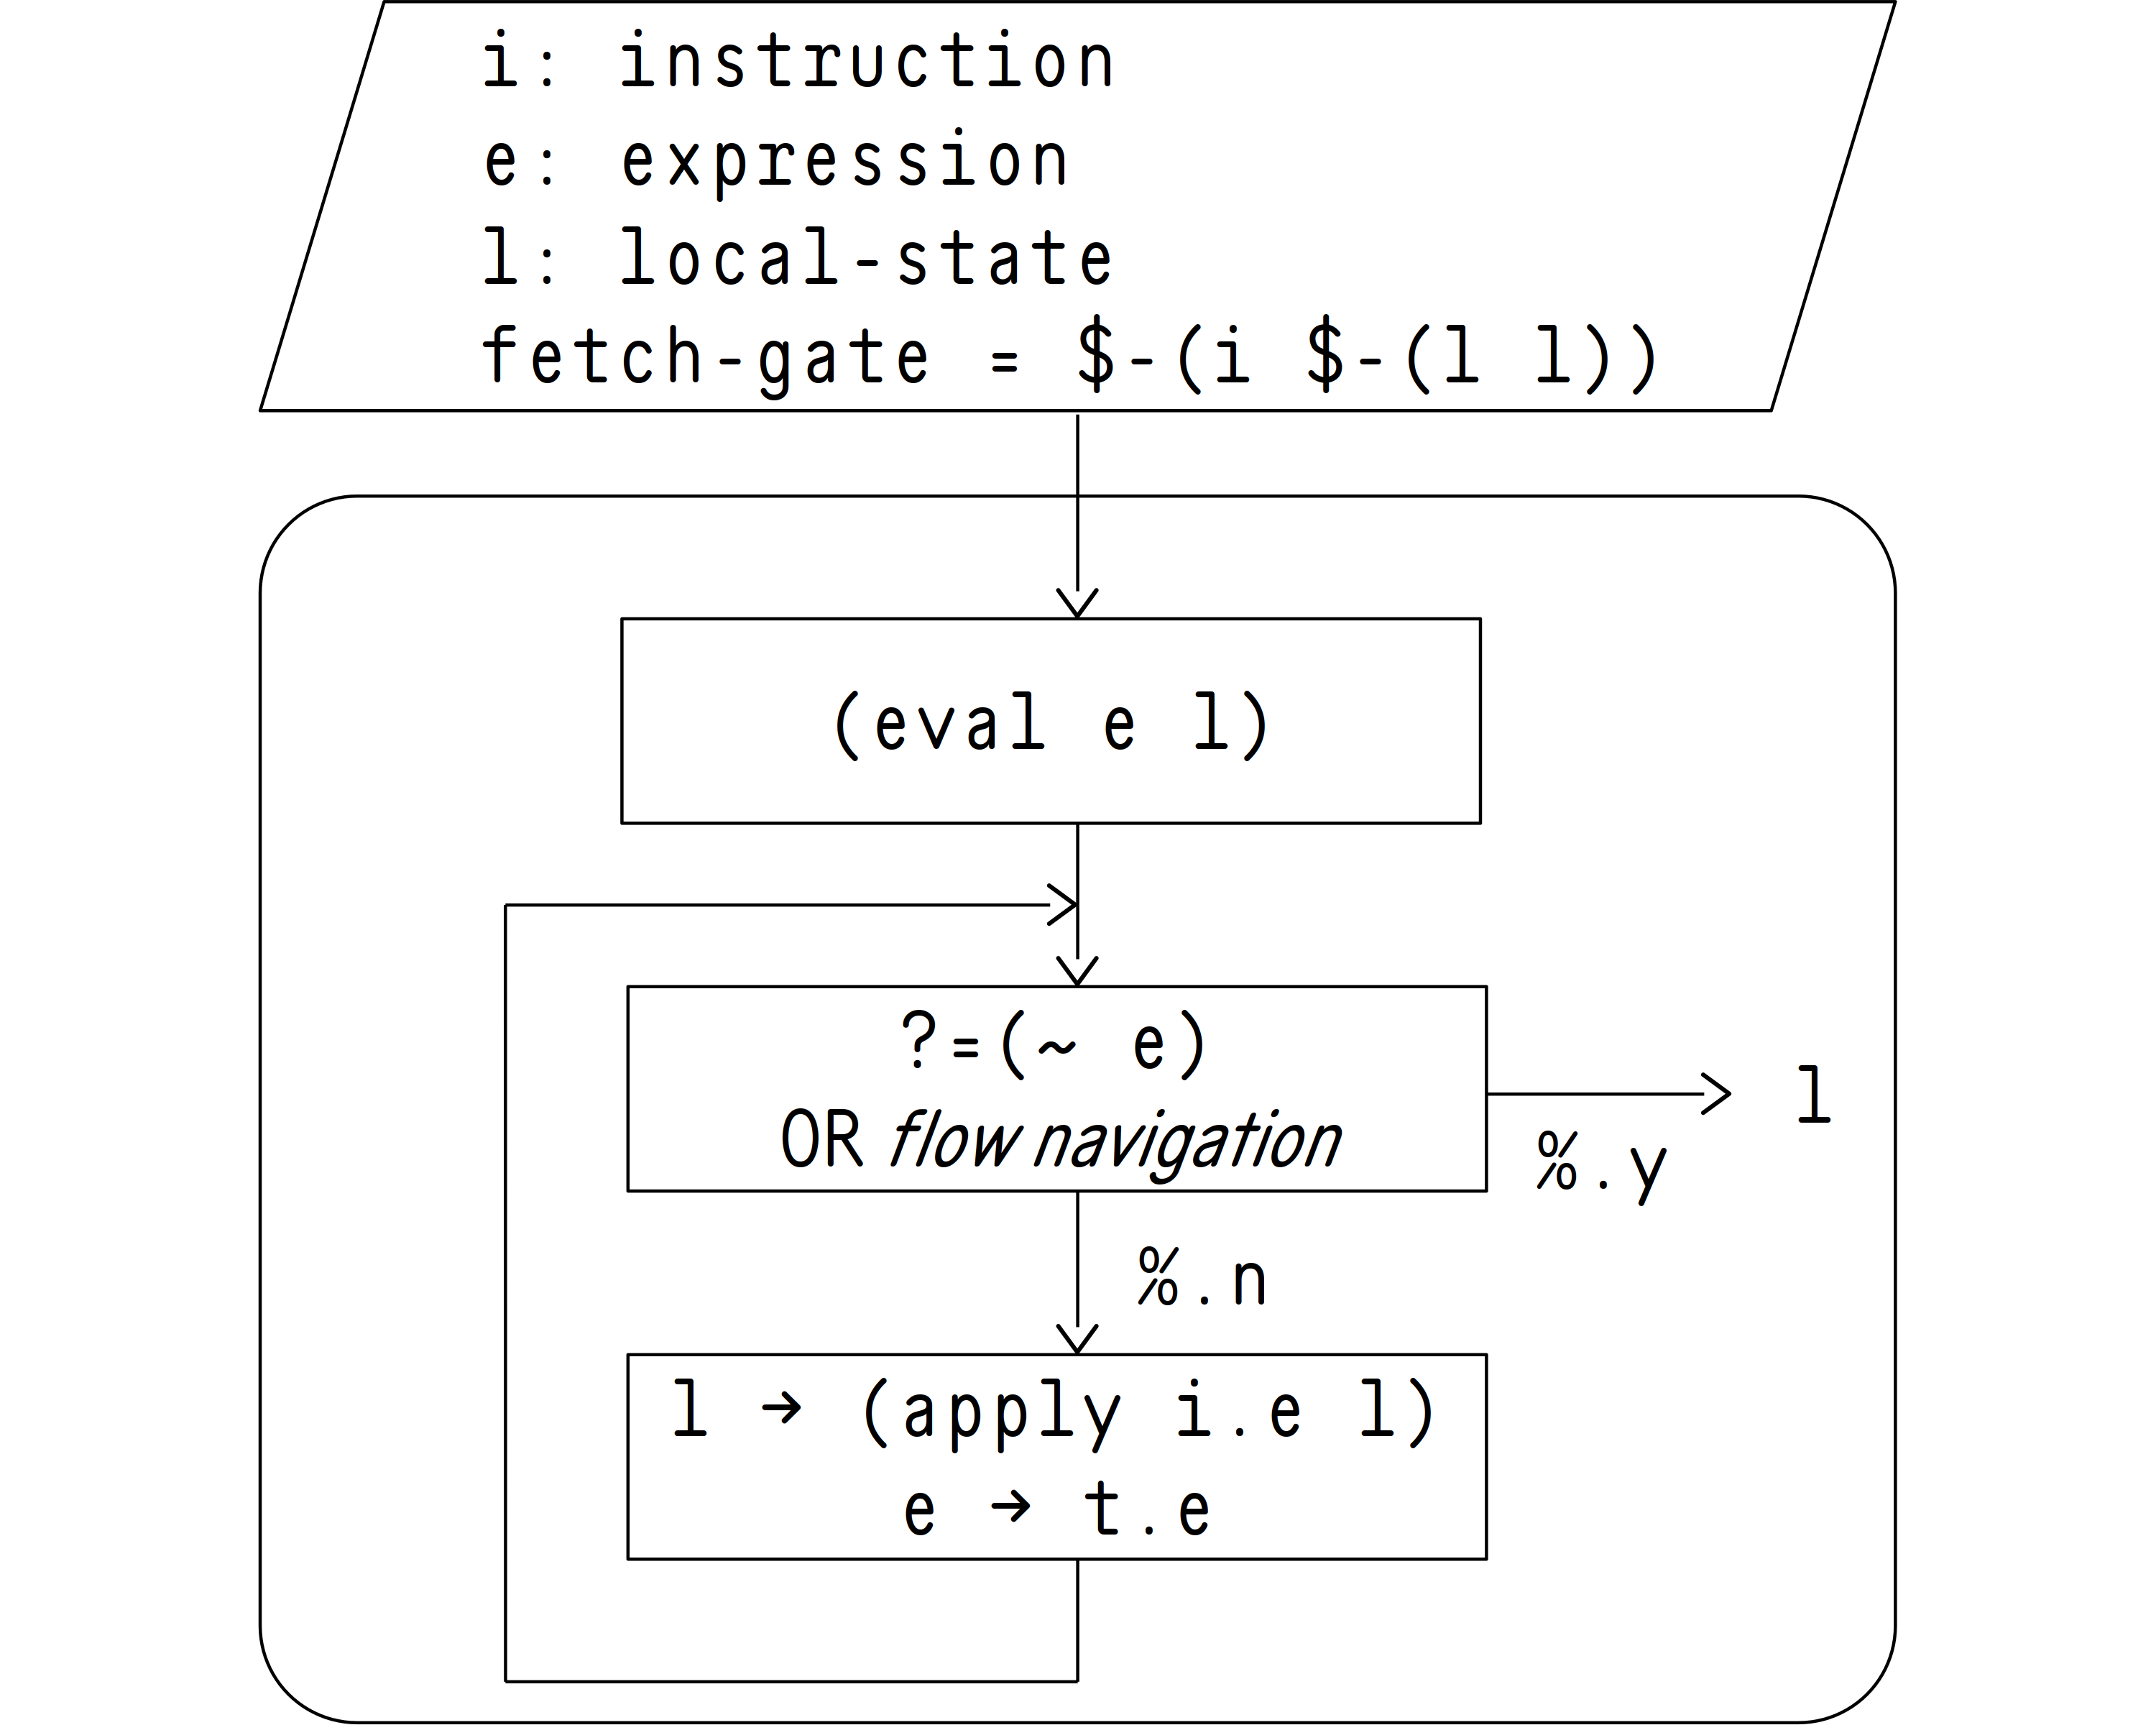
\includegraphics[width=\textwidth]{img/uw-eval}
    \caption{\lstinline[style=inlinecode]{++eval} data flow.}
    \label{fig:uw-eval}
  \end{subfigure}
  \\ ~ \\ ~ \\
  \begin{subfigure}{\textwidth}
    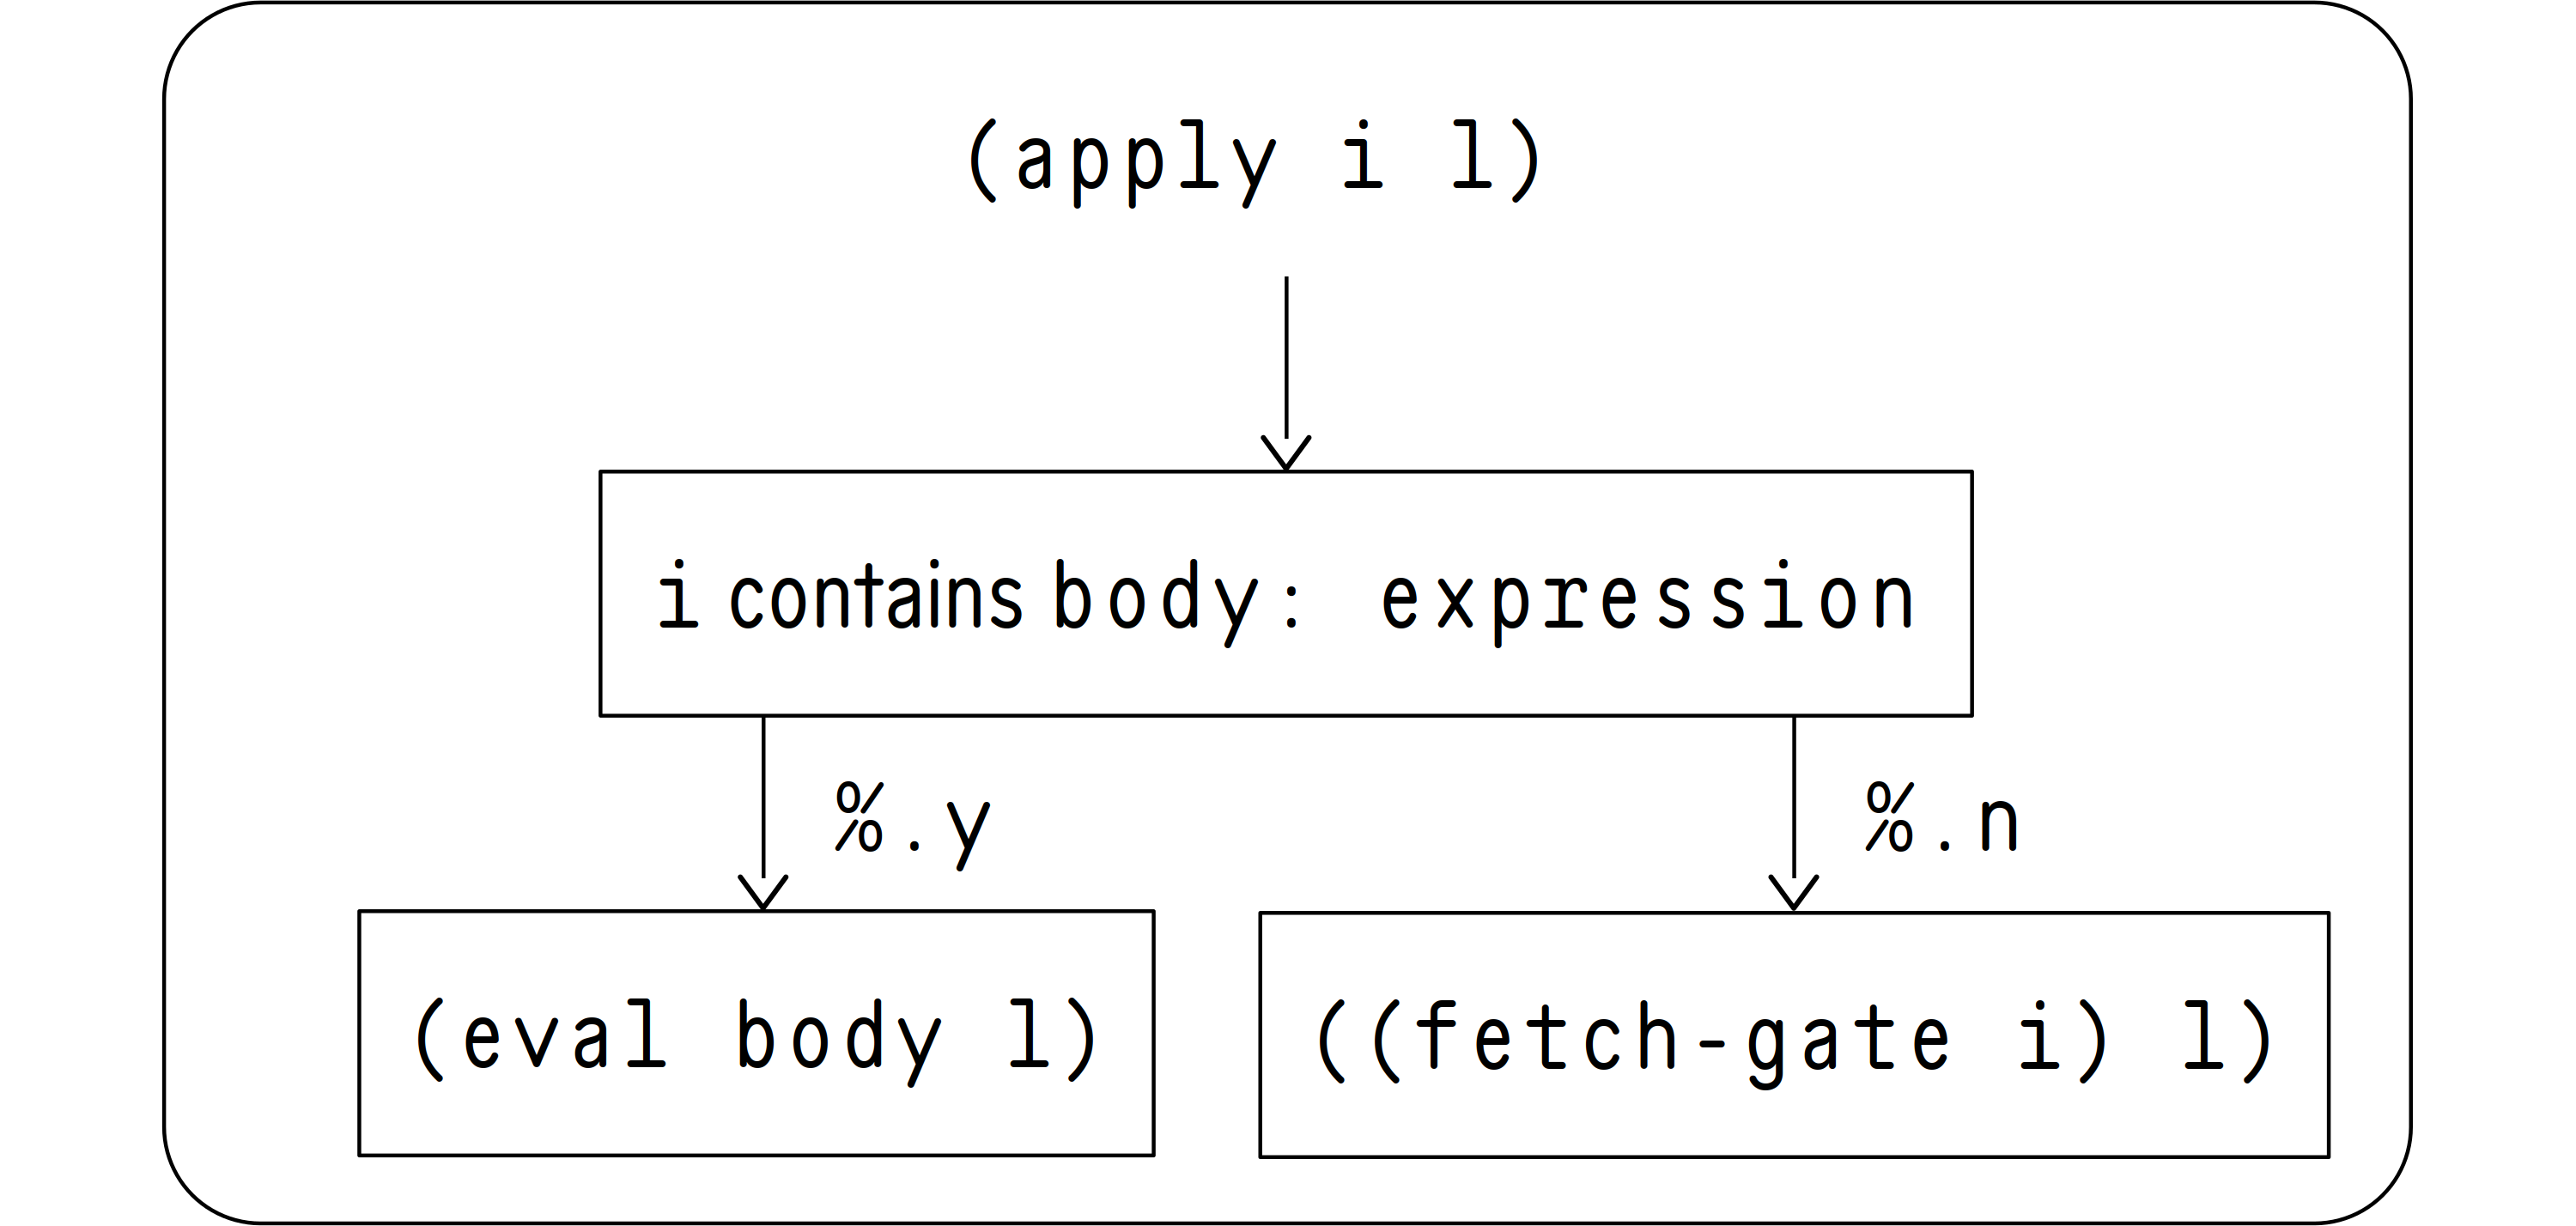
\includegraphics[width=\textwidth]{img/uw-apply}
    \caption{\lstinline[style=inlinecode]{++apply} data flow.  Some details like entering/exiting frames are elided.}
    \label{fig:uw-apply}
  \end{subfigure}
\caption{Data flow in the \texttt{urwasm} interpreter.}
\end{figure}

\sloppy
The gates above are internal; the outside caller will typically interact via two other gates, \lstinline[style=inlinecode]{++prep} and \lstinline[style=inlinecode]{++invoke}. \lstinline[style=inlinecode]{++prep} instantiates the module: it loads the data segments into the linear memory, instantiates global values, and runs a start function if specified. The product of this gate is either \lstinline[style=inlinecode]{global-state}, which describes the state of the Wasm module in between function invocations, or a block on an unresolved import, or a crash or “trap” in WebAssembly terms.

\lstinline[style=inlinecode]{++invoke} takes a name of an exported function, input values with type annotation and \lstinline[style=inlinecode]{global-state}. It performs a typecheck on the supplied values and calls an appropriate function. The result (as with \lstinline[style=inlinecode]{++prep}) either succeeds with output values and updated state, or blocks/traps.


\section{The WebAssembly VM and Determinism}

The state of an Urbit computer, as already mentioned above, is a pure function of its stream of events with the lifecycle function defined in Nock. No information other than the event log may impact the computation of this state, including the hardware on which the interpreter runs or the implementation details of the interpreter. For a Wasm interpreter in Nock to be practical it needs to be paired with some fast implementation of the Wasm interpreter in another language, and the equivalence of both algorithms must to be confirmed. In this way, the Urbit computer can be a practical personal server without violating its simple definition: the code of functions in Nock must be sufficient for an Urbit programmer to reason about the system.

This demand of equivalence, however, poses some difficulties. Some instructions of Wasm are defined non-determinis\-tically. For example, the \lstinline[style=inlinecode]{memory.grow} instruction can return -1 and not increase the length of the linear memory even if the maximum size of the memory described in the module file is not exceeded. The choice is left to the embedder, which can opt to keep the size of the memory buffer based on its resources.

In addition, some numerical operators return a set of values; that is, a Wasm VM could return any value from that set. This typically happens with floating-point operators when they are given a NaN value, with the set being defined by the value being a canonical NaN or not.\footnote{Cf. \citet{Davis2024}, pp. 93–131 in this issue.}  Some numerical operators return an empty set of values. In other words, their behaviour is set to be undefined for certain inputs, and those operators are described as partial. This can happen, for example, with the \lstinline[style=inlinecode]{idiv_N} operator when the second operand is equal to zero. The behaviour of Wasm VM is undefined in this case.

Therefore, the Wasm interpreter in \lstinline[style=inlinecode]{urwasm} describes a deterministic Wasm machine, limited to a subset of behaviors:

\begin{enumerate}
  \item  If an empty set of values must be returned, the interpreter “traps”:  it returns a deterministic error as a result, similar to \lstinline[style=inlinecode]{++mink};
  \item  If a set of values must be returned, then a single result from that set is returned. The choice is particular to each operator, but typically, if the set was a union of sets that depend on multiple input parameters, then the choice was made from the set given by the first parameter. (Refer to \lstinline[style=inlinecode]{/lib/op-def} for more information.)
  \item  \lstinline[style=inlinecode]{memory.grow} and similar instructions always attempt to grow the buffer when the limits in the module file permit.
\end{enumerate}


\section{Examples of \texttt{urwasm} Programs}

Some simple programs are included in the test suite. Most of them involve only numerical operations, while one of them calls a Wasm program compiled from Rust source which flips the order of characters in the string. Evaluation of this function requires multiple Wasm function invocations in order to e.g. allocate memory for the input string, and interaction with the global-state to read from and write to linear memory.

When Rust source is compiled, the compiler produces Java\-Script code which takes care of low-level handling of the state of Wasm runtime. In the case of Wasm interpreter in Hoon, JS code was manually translated to Hoon.

\sloppy
In addition, some other programs were run successfully. WebAssembly text format parsing in \texttt{urwasm} is implemented by composing the \texttt{wat2wasm} parser from the \texttt{wat} Rust crate with a binary parser in Hoon. Another example was presented at the Urbit Assembly in October 2023: an algorithm to simplify debts between a group of people, using the \texttt{FlowGraph} Dinic algorithm for maximum flow computation from the \lstinline[style=inlinecode]{contest_algorithms} Rust crate \citep{Afonin2023}.

These cited examples highlight the incredible inefficiency of the interpreter: it takes about a second to flip a string with 27 characters, and about a minute to parse a small Wasm binary with compiled \texttt{wat2wasm}. While there is most likely room for improvement, the Hoon code serves first and foremost as a formal specification of a deterministic Wasm VM, translated from the mix of pseudocode and mathematical formulas to a tightly-specified language. This specification would then serve for the verification of jet correctness.


\section{Jetting}

To jet the interpreter, the gate written in Hoon must be paired with a code in C that must be extensionally equivalent to the Hoon code. In that sense function definition in Hoon would act as a formal mathematical specification of what the interpreter returns, while C code would act as the actual implementation of Wasm runtime by arriving to the same conclusion as Hoon code but faster. The purpose of the Hoon specification is then to provide a test bed for verifying correctness of the interpreter, either by testing or formal analysis of both programs via e.g. the K verification framework (cf. \texttt{runtimeverification/ knock}, \citet{Hjort2023}).

Since Wasm is a portable language for a state machine, each invocation of a function from a Wasm module would either return a successful result with returned values and an updated state, or some flavor of failure (trap or blocking on unresolved external request, e.g. function call of an imported function). This gives us several possible strategies for jetting:

\begin{enumerate}
  \item  Have a bespoke Wasm interpreter in C that operates on nouns, and jet invoke gate.
  \item  Use an established Wasm runtime in C, and add serializer/deserializer to the jet, to convert Hoon representation of the module state to a representation in C and vice versa, and jet invoke gate.
  \item  Use an established Wasm runtime in C, and add serializer/deserializer to the Hoon specification, and use a representation of state close to the one in C as input and output in Hoon invoke gate, and jet invoke gate.
  \item  Don't jet the \lstinline[style=inlinecode]{++invoke} gate at all. Instead, have a higher level function that executes a series of operations on a module and doesn't return the entirety of Wasm module state. Hoon specification of this function would use the Wasm interpreter in Hoon, and the jetting code in C would use Wasm runtime in C.
\end{enumerate}

\noindent
But first, why do we have to have access to the state in the first place?

\begin{lstlisting}[
  float,
  style=listingcode_rust,
  caption={Rust function to reverse the order of characters in a string using Wasm.},
  escapeinside=``,
  label={lst:rust}
  ]
use wasm_bindgen::prelude::*;

#[wasm_bindgen]
pub fn process(input: String) -> String {
  let output_string: String = input.chars().rev().collect();
  output_string
}
\end{lstlisting}

Even for a simple source code the generated Wasm code might require multiple function invocations to get a desired result. Consider a Rust function that flips the characters in a given string (Listing \ref{lst:rust}).  After compiling this function to Wasm, you would get a module with five exported functions: \lstinline[style=inlinecode]{process} itself, \lstinline[style=inlinecode]{add_to_stack_pointer}, \lstinline[style=inlinecode]{malloc}, \lstinline[style=inlinecode]{realloc} and \lstinline[style=inlinecode]{free}.  The call of the compiled function in JS would look like:

\begin{lstlisting}[
  float,
  style=listingcode_js,
  caption={JavaScript function to reverse the order of characters in a string using Wasm.  Compare Listing~\ref{lst:rust}.},
  escapeinside=``,
  label={lst:js}
  ]
  export function process(input) {
  let deferred2_0;
  let deferred2_1;
  try {
    const retptr = wasm.__wbindgen_add_to_stack_pointer(-16);
    const ptr0 = passStringToWasm0(input, wasm.__wbindgen_malloc, wasm.__wbindgen_realloc);
    const len0 = WASM_VECTOR_LEN;
    wasm.process(retptr, ptr0, len0);
    var r0 = getInt32Memory0()[retptr / 4 + 0];
    var r1 = getInt32Memory0()[retptr / 4 + 1];
    deferred2_0 = r0;
    deferred2_1 = r1;
    return getStringFromWasm0(r0, r1);
  } finally {
    wasm.__wbindgen_add_to_stack_pointer(16);
    wasm.__wbindgen_free(deferred2_0, deferred2_1, 1);
  }
}
\end{lstlisting}

\noindent
Multiple invocations are necessary, some with the arguments received from outputs of other invoked functions. Having the access to the state of the module is thus crucial for any practical interpreter. In addition, we may have to read data from the state and save it as a noun, in order to perform I/O on that piece of information, since Arvo may only send effects when the computation of a given event has finalized. While jets could in theory perform system calls during their evaluation, doing so is considered a gross violation of jetting mechanism: jets as functions are supposed to be as pure as possible, to imitate their Nock definitions.

Let us review our options.

\subsection{Bespoke Wasm interpreter that operates on nouns}

Maybe this is the perfect option in the long term, but this option is unfeasible in the short to medium term due to the required development time. In addition, it would require speculative kinds of optimizations added to a Nock interpreter that do not yet exist, such as “data jets”, when a noun is represented in a way that allows certain operations faster to be performed faster. (For example, the Nock runtime could have a list of bytes \texttt{(list @D)} represented as a byte array in its memory, with some jetted functions configured to operate on that kind of nouns more efficiently.)

\subsection{Serialization/deserialization in the jet}

The next solution is to add serializer and deserializer functions to the jet of the \lstinline[style=inlinecode]{++invoke} arm, which would convert the noun representation of the state of the module to a representation legible to the jetting interpreter before evaluating the invoked function, and convert it back into a noun when the computation is finished. However, having to translate the state between two models twice for each function invocation would impose a lot of computational overhead.

\subsection{Serialization/deserialization in Hoon}

A less obvious variation is to put the de/serializer in the Hoon code of \lstinline[style=inlinecode]{++invoke}, and have the jetted gate take and return module state in the same representation as in the Wasm interpreter in C. The jet would then operate on the given state directly, without having to translate the state of the interpreter. Here the problem is that the implementation strategy leaks into the formal specification, making Hoon code jet-dependent. Replacement of the jetting Wasm runtime, including in the case of switching from Vere to Ares, would make us have to change the Hoon code, which I find to be antithetical to the Urbit project itself.

In addition, current model of jetting in both Vere and Ares requires that the core produced by the jetted arm is left read-only, without modification, so the output of the jet function cannot overwrite the core's sample. That would require the interpreter to copy the entire state of the module and operate on that, which creates prohibitive overhead for memory-heavy computations, like running a Linux VM.

\subsection{Higher level interpreter function}

This strategy would involve writing a function that takes a Wasm module, a list of operations to be performed and some other parameters, and then jetting this function. No intermediate state would be returned, saving us from having to convert it between different representations. However, a practical jet implementation would have to cache the intermediate state of the interpreter between Arvo events, otherwise it would have to reevaluate the operations each time the jetted function encounters a block on an unresolved import, or if the caller appended new operations to the list to interact with the module.


\section{Lia Interpreter}

Let's return to our example with string flipping in Rust. How would our hypothetical higher-level function run the program?  Ignoring imports for now, consider this gate:

\begin{lstlisting}[style=listingcode_rust]
++  lia
|=  [module=octs actions=(list action)]
^-  $%  [%0 out=(list value)]
        [%2 ~]
    ==
::  (...)
\end{lstlisting}

This gate accepts a binary file of a Wasm module and a list of actions to be performed, and returns either a list of values in the event of successful resolution, or an error. A value here is either a WebAssembly numerical value or a slice of the linear memory called \texttt{octs} in homage to Hoon. To flip a string, we would pass it the module file obtained from the Rust compiler and a list of actions obtained from parsing this code (ignoring \texttt{realloc} for simplicity), as shown in Listing \ref{lst:lia}.

\begin{lstlisting}[
  float=h,
  style=listingcode,
  caption={Lia function to reverse the order of characters in a string using Wasm.  Compare Listings~\ref{lst:rust} and \ref{lst:js}.},
  escapeinside=``,
  label={lst:lia}
]
# Lia (Language for Invocation of Assembly) scripting
#   language
# "add_to_stack_pointer", "malloc" and "process"
# are functions exported by the wasm module from Rust
# example above
#
string0 = "Hello world".to_octs
retptr = __wbindgen_add_to_stack_pointer(-16)
ptr0 = __wbindgen_malloc(string0.len, 1)
memory.write(string0, ptr0)
process(retptr, ptr0, len0)
i32 r0 = memory.read(retptr, 4)
i32 r1 = memory.read(retptr+4, 4)
return memory.read(r0, r1)
\end{lstlisting}

This code is written in Language for Invocation of Assembly (Lia for short). We imagine this language to have a very small specification:  its only purpose is to describe sequences of actions to be performed with a Wasm module. These include function invocation and memory reads and writes, as well as variable declarations, \texttt{for} loops and conditionals for expressivity.

Listing \ref{lst:lia} above is essentially identical to the JS example in Listing \ref{lst:js}. Ideally, Lia will be generated by the compiler itself, just like the JS code was also generated, with placeholders for input values, where the caller could insert their parameters.

A jet of \lstinline[style=inlinecode]{++lia} would have to perform the same operations but with an interpreter in C. However, considering the tiny specification for Lia, we do not foresee implementing the algorithm identically in both Hoon and C to be a challenge.

The Lia interpreter as described has been non-interactive; it takes a module and a list of actions and returns a result. But the WebAssembly module can and should be interactive: we want to invoke a function, perform some I/O based on the result, then invoke a function again etc. In addition, the module might contain imported functions, which we wish to resolve to provide I/O to the Wasm program.

Interacting with an instantiated module in the case of \lstinline[style=inlinecode]{++invoke} jetting is straightforward: the state of the module is a noun, and to interact with the state we would call various jetted gates that invoke functions and perform I/O on the store. Handling import function calls is also straightforward: \lstinline[style=inlinecode]{++invoke} might return a blocked result with the name of the imported function, which is then resolved in the embedding context, modifying state of the module if necessary. How would the same be achieved in a stateless fashion?

\begin{lstlisting}[
  float,
  style=listingcode,
  caption={Upgraded \texttt{++lia} arm.},
  escapeinside=``,
  label={lst:lia2}
]
++  lia
  |=  $:  module=octs
          actions=(list action)
          shop=(list (list value))
          ext-func=(map (pair cord cord) (list action))
          diff=(each (list action) (list value))
      ==
  ^-  $%  [%0 out=(list value)]
          [%1 name=path args=(list value)]
          [%2 ~]
      ==
  =>
    ?:  ?=(%.y -.diff)
      .(actions (weld actions p.diff))
    .(shop (snoc shop p.diff))
  ::  (...)
\end{lstlisting}

In Listing~\ref{lst:lia2}, we have added details to the block or trap.  Now the interpreter can return a block with \lstinline[style=inlinecode]{%1}, asking for an external reference to be resolved and the result of the resolution to be appended to shop. The interpreter now takes a list of list of values \lstinline[style=inlinecode]{shop}, which represents the resolved Lia imports; \lstinline[style=inlinecode]{ext-func}, which provides definitions for imported functions for a given Wasm module; and \lstinline[style=inlinecode]{diff}, whose contents are appended to an appropriate field.

Notice the difference between imports in Lia and in Wasm: the namespace of the latter is defined with a pair of strings in compliance with the formal specification, and the input parameters of \lstinline[style=inlinecode]{++lia} contain definitions of the imported functions for the Wasm module. Lia imports, on the other hand, are bound to a path namespace and are external to \lstinline[style=inlinecode]{++lia}.

In a trivial case the list of actions of a function definition in ext-func would contain a single call to a function which is external to Lia and is named with \lstinline[style=inlinecode]{path}, not \lstinline[style=inlinecode]{(pair cord cord)} like Wasm import functions. In a nontrivial case the list of actions could contain multiple actions to be performed, e.g. a memory read followed by calling a Lia \lstinline[style=inlinecode]{import} function which takes \lstinline[style=inlinecode]{octs}. The purpose here is for the \lstinline[style=inlinecode]{import} calls to be able to surface not only Wasm values but Lia values like \lstinline[style=inlinecode]{octs}, giving us the richness of import calls that we could have with \lstinline[style=inlinecode]{++invoke} jetting model without exposing the entirety of the module's state.

\subsection{Caching of store}

Since Wasm execution is deterministic, then the state of a module, whether in Nock or in the jetting environment, is referentially transparent with regards to the input parameters of Lia. Here \lstinline[style=inlinecode]{diff} appears to be semantically useless, since instead of placing changes there we could have placed them directly into a proper field of the sample.

But \lstinline[style=inlinecode]{diff} is necessary for efficient computations: each time \lstinline[style=inlinecode]{++lia} jet computes something with a Wasm runtime, it will save a cache of Lia interpreter in the jetting environment tagged with a (hash of a) noun \lstinline[style=inlinecode]{[module actions shop ext-func]}. If \lstinline[style=inlinecode]{++lia} is computed later with the same first four arguments, then the jet would first look for a cache, and if it finds one, only compute the diff, either injecting results of Lia import resolution into a suspended jetting Lia interpreter, or performing a list of appended actions. Failing to find a cache, jet of \lstinline[style=inlinecode]{++lia} would do the same thing as \lstinline[style=inlinecode]{++lia} in Hoon: append the \lstinline[style=inlinecode]{diff} to an appropriate field and run the whole thing.

At the price of having to bother with cache reclamation and perhaps slightly longer event log replays we get the possibility of running Wasm runtime almost full speed, without having to de/serialize nouns to structs and vice versa or to copy the state of the Wasm module for every interaction with it. In Nock the state of the Wasm module is represented lazily with the first four parameters of \lstinline[style=inlinecode]{++lia}, while the actual state on which we perform computations exists as a cache.

A typical interaction with \lstinline[style=inlinecode]{++lia} would look like this:

\begin{enumerate}
  \item  Call \lstinline[style=inlinecode]{++lia} for the first time, with an empty diff.
  \item  Lia returns one of:
  \begin{enumerate}
    \item  success \lstinline[style=inlinecode]{%0};
    \item  block \lstinline[style=inlinecode]{%1}; or
    \item  failure \lstinline[style=inlinecode]{%2}, which is resolved outside of Lia.
  \end{enumerate}
\end{enumerate}

\noindent
The resolution result is placed into \lstinline[style=inlinecode]{diff}, and \lstinline[style=inlinecode]{++lia} is called again. Next time that same result must be placed directly to shop to get the right cache and avoid recalculating from scratch.

If the result is success, new actions can be put in diff and \lstinline[style=inlinecode]{++lia} can be called again to continue interacting with the module. After that these new actions must be placed directly to actions on subsequent calls of \lstinline[style=inlinecode]{++lia} to get the right cache.

As for the cache reclamation, \lstinline[style=inlinecode]{++lia} could include another input parameter hint ignored in Hoon code, that would serve as a hint to the jet on how to handle the cache, e.g. for how long to keep it in the memory. Dojo generators and Gall agents, for example, would likely benefit from different cache reclamation strategies.


\section{Next Steps}

What is the roadmap forward for the \texttt{urwasm} project?  The first priority is to add unit tests and module validation in Hoon.  This will allow us to verify the correctness of the interpreter and to ensure that the jetting process is successful.  The next stage will consist of enabling caching in the jet of \lstinline[style=inlinecode]{++lia} and adding a parser from text to \lstinline[style=inlinecode]{(list action)}.  This will enable us to construct a Lia interpreter in Hoon, jetted with the Lia interpreter in C/Rust.  This facilitates a default Gall agent interface to interact with Lia and enable building Gall apps in conventional languages.  Finally, we will add Wasi support and Lia generation to common Wasm compilers in the same way they generate JS wrappers for the modules.


\section{Conclusion}

This paper presents a novel method of modeling state machines in Nock and jetting the associated modeling algorithm. In this method the state is represented implicitly through a list of actions performed on the initialized state of the machine, and the state of the jetting emulator of the state machine is kept as a cache identified with the list of actions. This gives the interpreter full computational speed due to lack of overhead caused by translating the state from noun representation to the jetting representation and back and by the fact that the jetting function is free to edit the state in place, as long as it updates the naming tag of the cache.  \tombstone{}

\selectlanguage{USenglish}
\printbibliography
\end{document}
